\chapter{Search Strategy}
\label{ch:SearchStrategy}

\section{Physics Objects}\label{PhysObj}
There are many different types of physics objects that we are interested in when working with particle physics experiments. Since the particles that we are interested in have very short lifetimes, $\mathcal{O}(\text{decay})=10^{-23}$ s, we mainly interact with the decay products of the event, such as, jets $(N_j)$, heavy object tagging $(\nt, \nw, \nrt)$, missing transverse momentum (\met), sum scalar jet momentum $(H_T)$, number of secondary vertices $(N_{SV})$, transverse momentum of leading $b$ jet $(\pt^b)$, transverse mass between tagged $b$ quarks amd \met{} $(m_T(b_{1,2}, \met))$, Initial State Radiation, and lepton identification.

\subsection{Jets}\label{Jets}
In an interaction whenever a quark is made it must come in pairs $(q\overline{q})$ such that the total color and electric charge of the interaction is neutral. Typically due to conservation of momentum the quarks may originally be produced near the interaction point but will quickly start to move away from each other. Eventually the quarks will move far enough apart and will have enough potential energy in the gluon connections between them that it is now more efficient to create a new quark-antiquark $(q\overline{q})$ pair. This will continue to occur in a sequence of radiating gluons and producing new pairs of charged particles. In the final state, the energy deposited in the HCAL is due to a cluster of charged particles of a certain radius, $\Delta R=\sqrt{\Delta\eta^2+\Delta\phi^2}$. There are many algorithms to reconstruct the jets, we are mainly interested in the anti-kT Jet algorithm \cite{cacciari_anti-ktjet_2008} method which uses the transverse momentum of the particles within a certain radius $\Delta R = 0.4 (0.8)$ for AK4(AK8) jets \cite{noauthor_jetid_nodate, noauthor_jec_nodate}. Once the jets have been identified, we cause analyse their respective properties to determine the likelihood of the particle it originated from, such as a $b, t, \text{ or } W$. 

\begin{figure}
 	\centering
	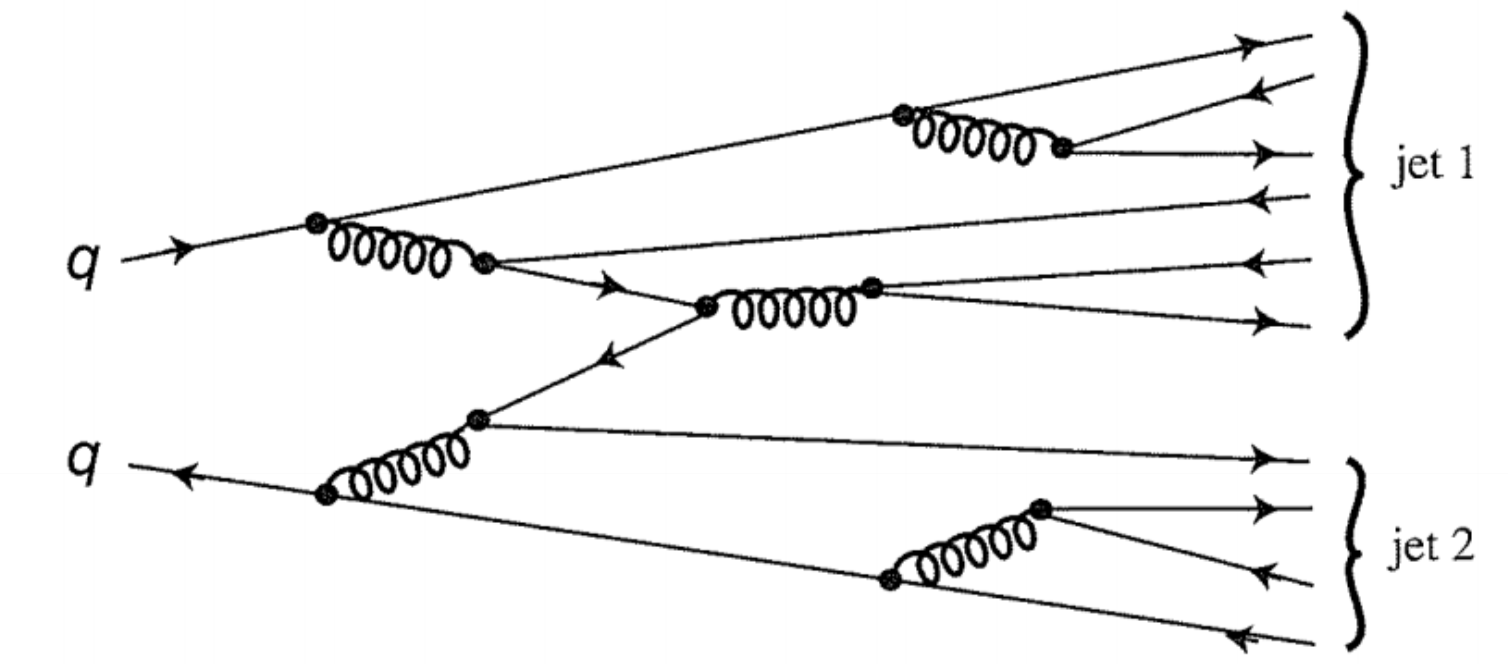
\includegraphics[width=0.75\textwidth]{JetHadronization.png}
 	\caption[Jet Hadronization]{A diagram of a quark pair radiating gluons that decay into more quark pairs in a process called hadronization \cite{griffiths_introduction_2008}.}
 	\label{JetHadronization} 
\end{figure}

\subsection{Heavy Object Tagging}\label{HeavyObject}
Since this search is looking for a massive particle which then decays to slightly less massive particles we need to be able to identify and distinguish between them. We use various algorithms and neural networks to identify jets from $b$ quarks, \bjet s or from $t$ quarks. 

\subsubsection{B-Tagging}\label{Btagging}
Firstly, \B-tagged jets which are jets that are likely to have originated from a \B{} quark. These are identified reconstructing where the jet originated from and comparing the distance away from the interaction point. A \B{} quark is a relatively long-lived particle and can travel many millimeters before decaying. Since we have a resolution of \mum{} this is not a problem. For \B{} quarks with large transverse momentum, we use a Deep Combined Secondary Vertex (DeepCSV) algorithm that involves neural networks. 

\bjet s{} are identified using the Run 2 version of the Deep Combined Secondary Vertex (DeepCSV) algorithm. The medium working point recommended by the B-tag POG, corresponding to a threshold of 0.6324m 0.4941, and 0.4184 for the 2016, 2017, and 2018 respectively \cite{noauthor_btagrecommendation2016legacy_nodate, noauthor_btagrecommendation94x_nodate, noauthor_btagrecommendation102x_nodate}.

\begin{figure}
 	\centering
	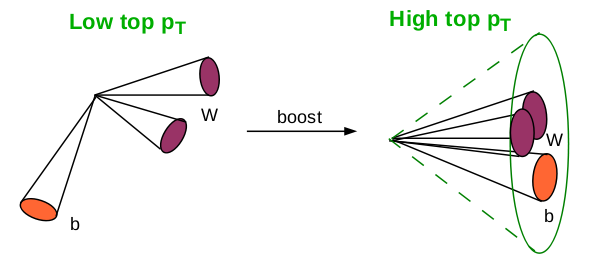
\includegraphics[width=0.75\textwidth]{TopDecayBoost.png}
 	\caption[Top Decays]{The two types of top quark reconstuctions, when each decay product is easily identifiable (resolved) or when the particles are close together (boosted).}
 	\label{TopDecays} 
\end{figure}

\subsubsection{Top/W Tagging}\label{TopTagging}
The anti-kt algorithm using a distance parameter, $\Delta R=0.8$, is expected to contain the energy clusters of all of the decay product of boosted $t$ quarks, see Fig. \ref{TopDecays}, with $\pt>300$ \GeV or \W bosons with $\pt>200$ \GeV. The requirements are:
\begin{itemize}
	\item Medium working point $>0.937, 0.895, 0.895 (0.973, 0.991, 0.991)$ for boosted $t$ $(W)$ for the separate 2016, 2017, and 2018 eras, respectively.
	\item Reconstructed soft drop mass: $105<m_t<210$ \GeV{} and $65<m_W<105$ \GeV.
	\item Boosted tops: $\pt=300$ \GeV, $|\eta|<2.0$ and $W$: $\pt=200$ \GeV, $|\eta|<2.0$
\end{itemize}

There is another type of top that can be reconstructed, which is when each subjet of the top decay can be resolved into each individual jet, denoted as a resolved top, see Fig. \ref{TopDecays}. The requirements are:
\begin{itemize}
	\item Medium working point: 0.92 for all eras.
	\item $|\eta(j_{1,2,3})|<2.4$ and $b$-tag desciminator: $>0.6324, 0.4941, 0.4184$ for the separate 2016, 2017, and 2018 eras, respectively. The number of jets that pass these cuts should be $\geq2$.
\end{itemize}
These object definition are orthogonal to each other and are used to bin our search and control regions. 

\subsection{Missing Transverse Momentum}\label{MET}
The missing transverse momentum is the negative vector sum of the total transverse momentum measured in the detector,
\begin{equation}
\met=-\sum_{i\in\text{vis}}\overrightarrow{p}_{i, T},
\end{equation}
where the momentum runs over every visible(vis) particle in the event. Ideally, if the detector was $100\%$ this quantity would always be zero due to conservation of momentum, but many things, such as detector efficiency, paticles that are weakly interacting, or particles beyond the SM will cause the missing energy. Because of these, this object is a good discriminator for searching for physics beyond the SM. 

\subsection{MET Filters}
Need to add MET Filters here.

\subsection{$H_T$}\label{HT}
Another interesting quantity is $H_T$, which is the scalar sum of the \pt of all of the jets in an event,
\begin{equation}
H_T=\sum_{i\in\text{jets}}p_{i,T}.
\end{equation}
This quantity is quite useful when trying to identify massive particles and is quite good at suppressing QCD multijet background.

\subsection{Soft $b$-Tagging}\label{SV}

The ability to identify secondary vertices is essential in searches for the top squark, see Sec. \ref{sec:Production}. Since the b quark is a long lived particle, about $10^{-12}$ seconds, that will travel many millimeters before decaying into other particles. The displaced vertex of the long lived $b$ quark is reconstructed from the tracks that it produces in the detector. We then reconstruct the tracks to a point that is displaced from the primary vertex $(PV)$ it is known as a secondary vertex $(SV)$ and has the potential to be an long lived particle. 

\begin{figure}
 	\centering
	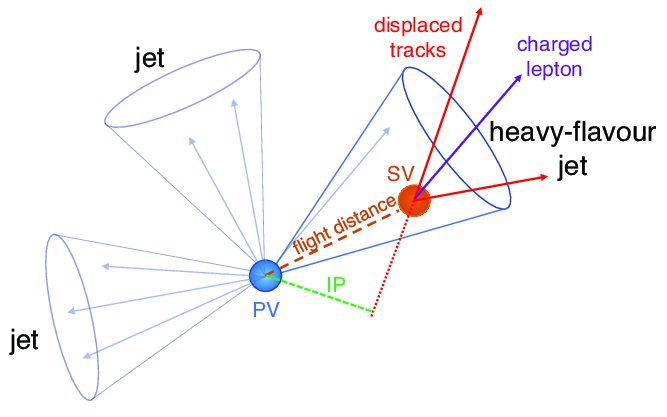
\includegraphics[width=0.75\textwidth]{SecondaryVertex.png}
 	\caption[Secondary Vertex Diagram]{A interaction that produces a long lived particle that has a reconstruced SV.}
 	\label{SecondaryVertex} 
\end{figure}

This search targets also models that produce very soft bottom or charm quarks. A large fraction of events contain b quarks with \pt{} below the 20 GeV jet \pt{} threshold which may thus fail to be reconstructed as jets or become b-tagged. Identification of these soft quarks improves our ability to separate potential signal events from the SM background. We therefore aim to identify b/c quarks based on the presence of a SV reconstructed using the Inclusive Vertex Finder (IVF) \cite{noauthor_inclusivesecondaryvertexfinder_nodate}. Additional requirements on SV observables are applied to suppress the background originating from light quarks. These selected SV may be referred to as soft $b$-tags and are constructed to be orthogonal to the jets and b-tagged jet used in this analysis. 

The requirements on each SV to pass the soft b-tagging definition are:
\begin{itemize}
	 \item The distance in the transverse plane between the SV and the PV $\leq3$ cm.
	 \item The significance of the distance, SIP3D, between the SV and thePV $\geq4$.
	 \item The pointing angle, defined as $cos(\overrightarrow{PV,SV},\overrightarrow{p}_{SV})\geq0.98$, where $\overrightarrow{p}_{SV}$ is the total four-momentum of the tracks associated to the SV. 
	 \item The number of tracks associated to the SV is greater or equal to 3.
	 \item The \pt{} of the SV is less than 20 GeV.
\end{itemize}

\subsection{Initial-state Radiation}\label{ISRpt}

Initial-state radiation (ISR) may be clustered into one of the large-$R$ jets clustered with a distance parameter, $\Delta R=0.8$. We use the larger radius jets to be sensitive to ISR with gluon splitting, when a jet radiates a qluon that pair produces two quarks. The ISR jet is identified as being the hardest of the large-$R$ jets with $\pt>200$ GeV which fails the loose b-tagging working point and is not identified as a top or W. 
 
 \subsection{Lepton Identification}\label{EleMuonID}
 There are two sets of selection criteria used in the analysis for electrons and muons. A set of veto criteria are used to efficiently reject events with an isolated electron of muon in the search region, while more stringent requirements are imposed in some control regions that require high purity samples of isolated leptons.
 
 Electron candidates are identified via a set of selection criteria established by the EGamma POG based on "Spring16" simulated samples in the 25ns bunch spacing scenario. The corresponding thresholds imposed on relevant variables are summarized in Table . The "Veto" working point is used to keep events with electrons out of the final search region. The "Medium" working point is used for the selection of leptonic control regions. 
 
 \begin{table}
 \centering
 \begin{tabular}{|*{5}{c|}}
 \hline
 \multirow{2}{*}{} & \multicolumn{2}{c}{Veto Working Point} & \multicolumn{2}{c}{Medium Working Point} \\
 \hline
 & Barrel & Endcap & Barrel & Endcap \\
\hline
$\sigma_{i\eta i \eta} (\text{full} 5 \times 5) <$ & 0.0114 & 0.0352 & 0.0101 & 0.0283 \\
$|\Delta\eta_{\text{in}}|<$ & 0.0152 & 0.0113 & 0.0103 & 0.00733 \\
$|\Delta\phi_{\text{in}}|<$ & 0.216 & 0.237 & 0.0336 & 0.114 \\
$\frac{h}{E} <$ & 0.181 & 0.116 & 0.0876 & 0.0678 \\
$\frac{1}{E}-\frac{1}{p}<$ & 0.207 & 0.174 & 0.0174 & 0.0898 \\
$|d_0|<$ & 0.0564 & 0.222 & 0.0118 & 0.0739 \\
$|d_z|<$ & 0.472 & 0.921 & 0.373 & 0.602 \\
$N(\text{expected missing inner hits})\leq$ & 2 & 3 & 2 & 1 \\
Conversion veto & pass & pass & pass & pass \\
\hline
 \end{tabular}
 \caption[Electron Identification Parameters]{Electron identification requirements, defined separately for electrons in the ECAL barrel and endcap regions. The tabulated numbers for each working point are the thresholds applied to the corresponding quantities in the first column.}
 \label{ElectronID}
 \end{table}
 
 The loose muon definition recommended by the Muon POG is used for the purposes of the muon veto. A loose muon is identified as a PF muon and can be either a global muon or an arbitrated tracker muon. Only candidates with transverse (longitudinal) impact parameter $|d_0|<0.2$ cm $(|d_z|<0.5 \text{cm},)$ with respect to the primary vertex, are considered. The muon selection in leptonic control regions relies on the medium working point defined by the Muon POG for higher purity. The medium muon requirements are summarized in Table . They are applied in addition to the loose muon requirements. Selected muons are required to have transverse (longitudinal) impact parameters $|d_0|<0.05$ cm $(|d_z|<0.1 \text{cm}),$ with respect to the primary vertex. 

\begin{table}
 \centering
 \begin{tabular}{|*{2}{c|}}
 \hline
Loose muon selection & yes \\ 
Fraction of valid tracker hits & $> 0.8$ \\
\hline
\hline
\multicolumn{2}{c}{In addition, either of the following sets of requirements:} \\
\hline
Global muon & yes \\
Normalized global-track $\chi^2$ & $< 3$ \\
Tracker-Standalone position match & $< 12$ \\
Track kink finder & $< 20$ \\
Segment compatibility & $>0.303$ \\
\hline
\multicolumn{2}{c}{OR} \\
\hline
Segment compatibility & $> 0.451$ \\
\hline
 \end{tabular}
 \caption[Muon Identification Parameters]{The requirements for a particle trajectory to be tagged as a muon. }
 \label{MuonID}
 \end{table}
 
 The isolation requirements used in the selection of electrons and muons aim to achieve a high efficiency for correctly identifying events that contain prompt leptons (i.e. leptons that do not originate from heavy flavor decays) in the boosted topologies and busy hadronic environments that are typical for this analysis. They are based on the mini-isolation quantity, which is a measure of the lepton's local isolation. Mini-isolation is computed as the summed \pt of PF candidates within a $\Delta R$ cone centered on the lepton candidate. The cone size depends on the lepton \pt as indicated in Table  and is intended to be small enought to reduce overlaps with jets in the event while also being large enough to contain the products of leptonic b-decays. Higher values of instantaneous luminosity result in a reduced efficiency for the isolation requirement due to an increase in the number of particles originating from additional (pileup) interactions that enter the isolation cone. In order to minimize this effect, the calculated isolation quantity is corrected for the estimated contribution from pileup particles. The correction is applied by subtracting the product of the estimated average pileup density $(\rho)$ in the event with an effective area, $A_{eff}$, related to the geometrical size of the isolation cone. The residual dependence of the isolation quantity on $\rho$ for a given cone size is accounted for in $A_{eff}$, which is determined by taking the slope of a linear fit to the uncorrected isolation as a function of $\rho$. The correction factor is $\eta$-dependent, and calibrated separately for charged particles, neutral hadrons, and photons contributing to the isolation. 
 
 Electrons and muons are considered to fulfill the veto isolation criteria if their mini-isolation is less than 0.1 or 0.2 respectrively, relative to the lepton \pt. The same thresholds are applied on the relative mini-isolation for electrons and muons in control samples. 
 
\subsection{Tau Identification}\label{TauID}
The Tau ID has been studied extensively. After multiple studies which looked into the custum MVA similar to the one used in [], the IsoTrack methods, and Tau POG MVA method of Identifying Taus. The methods which provide the best improvement to the efficiency of identifying taus with a small fake rate is the combination of IsoTrack and Tau POG MVA. With the inclusion of the combined method for identifying hadronically decaying taus the efficiency should improve greatly. 

\section{Search Strategy}\label{BaselineSearch}


\subsection{Trigger}
The following filters, recommended by the JetMET POG, are applied to 2016, 2017, and 2018 eras:
\begin{itemize}
	\item goodVertices
	\item HBHENoiseFilter
	\item HBHENoiseIsoFilter
	\item EcalDeadCellTriggerPrimitiveFilter
	\item BadPFMuonFilter
	\item GlobalSuperTightHalo2016Filter
	\item eeBadScFilter
\end{itemize}
There is an addition ecalBadCalibFilter for 2017 and 2018 eras only.

\subsection{Baseline Selection} \label{Baseline}

Following the same methods as above, we have a loose pre-selection which is refered to as the baseline selection. This will place a selection on jets and \met which is used to eliminate a large fraction of background events. We define the baseline selection as:
\begin{itemize}
	\item $N_{e,(\mu)} = 0, (\pt>5$ \GeV, $|\eta|<2.5(2.4))$
	\item $N_{iso} = 0, (\pt > 5 (10)$ \GeV, ISO $< 0.2(0.1) \text{ for electron/muons(pions)})$
	\item $N_{tau} = 0, (\pt > 20$ \GeV, $|\eta|<2.4)$
	\item $N_{j} \geq 2, (\pt >20$ \GeV, $|\eta|<2.4)$
	\item $\met >250$ \GeV, to reach the plateau of the trigger efficiency
\end{itemize}
In Addition to this, we allow for two separte sets of additional selections to apply to the low and high \dm{} search regions to further reduce background. The high \dm{} baseline selection includes the baseline selection and additionally,
\begin{itemize}
	\item $N_j\geq 5, (\pt >20$ \GeV, $|\eta|<2.4)$
	\item $N_b\geq 1, (\pt >20$ \GeV, $|\eta|<2.4)$
	\item $\text{Min}[|\Delta\phi(\met,j_1)|,|\Delta\phi(\met,j_2)|,|\Delta\phi(\met,j_3)|,|\Delta\phi(\met,j_4)|]\equiv\Delta\phi_{1234}>0.5$, where $j_1, j_2, j_3, j_4$ are the four leading jets in $p_T$. This requirement is to reduce the QCD multijet background. 
\end{itemize}
Next, the low \dm{} baseline selection has the following addition selections,
\begin{itemize}
	\item $N_t=0, N_W=0,N_{res}=0,$ where $N_t$ and $N_W$ are the number of merged tops and \W's, respectively, and $N_{res}$ is the number of resolved tops
	\item An ISR jet is defined in Sec. \ref{ISRpt} with $\pt(ISR)>200$ \GeV, $|\eta|<2.4, |\Delta\phi(j_{ISR},\met)|>2.$
	\item $\met/\sqrt{H_{T}}\equiv S_{\met}>10$, where $H_T$ is calculated as the scalar sum of the \pt of jets with $\pt >20$ \GeV{} and $|\eta|<2.4.$
	\item $|\Delta\phi(\met,j_1)|>0.5, |\Delta\phi(\met,j_{2,3})|>0.15$, where $j_1,j_2,j_3$ are the three leading jets in \pt. 
\end{itemize}
\begin{table}[!ht]
\begin{center}
\caption[High $\Delta$m Search Regions]{\label{tab:searchregions-hm}Summary of the 130 disjoint search regions that mainly target high \dm~signal models. The high \dm~baseline selection is again $\nj \geq 5$, $\met>250~\GeV$, $\nb\geq1$, and $\dphijonetwothreefour>0.5$.}
\resizebox*{1\textwidth}{!}{

\begin{tabular}{|c|c|c|c|c|c|c|}
	\hline
	\multicolumn{7}{|c|}{$\mtb<175$\,\GeV}  \\
	\hline
	\nj				 & \nb				& \nt			   & \nw				 & \nrt				& \Ht ~[\GeV]		   & \met~[\GeV] 		\\
	\hline
	$\geq7$		& $1, \geq2$  & $\geq0$		 & $\geq0$			& $\geq1$	  & $\geq300$			& $250-300$, $300-400$, $400-500$, $\geq500$ \\
	\hline
	\multicolumn{7}{|c|}{$\mtb\geq175$\,\GeV}  \\
	\hline
	\nj				 & \nb				& \nt			   & \nw				 & \nrt				& \Ht ~[\GeV]		   & \met~[\GeV] 		\\
	\hline
	$\geq5$		& $1,\geq2$   &	$0$				& $0$				   & $0$			 & $\geq1000$		 & $250-350$, $350-450$, $450-550$, $\geq550$ \\
	\hline
	\multirow{6}{*}{$\geq5$} & \multirow{6}{*}{$1$} & $\geq1$ & $0$ & $0$ & $300-1000$, $1000-1500$, $\geq1500$ & $250-550$, $550-650$, $\geq650$\\
						  &					   & $0$			 & $\geq1$			& $0$			  & $300-1300$, $\geq1300$ & $250-350$, $350-450$, $\geq450$ \\
						  &					   & $0$			 & $0$				    & $\geq1$	  & $300-1000$, $1000-1500$, $\geq1500$ & $250-350$, $350-450$, $450-550$, $550-650$, $\geq650$ \\
						  &					   & $\geq1$	 & $\geq1$			& $0$			  & $\geq300$ 			& $250-550$, $\geq550$ \\
						  &					   & $\geq1$	 & $0$					& $\geq1$	  & $\geq300$			& $250-550$, $\geq550$ \\
						  &					   & $0$			 & $\geq1$			& $\geq1$	  & $\geq300$			& $250-550$, $\geq550$ \\
	\hline
	\multirow{10}{*}{$\geq5$} & \multirow{10}{*}{$2$} & $1$ & $0$ & $0$ & $300-1000$, $1000-1500$, $\geq1500$ & $250-550$, $550-650$, $\geq650$\\
						  &					   & $0$			 & $1$					& $0$			& $300-1300$, $\geq1300$ & $250-350$, $350-450$, $\geq450$ \\
						  &					   & $0$			 & $0$				    & $1$	  		& $300-1000$, $1000-1500$, $\geq1500$ & $250-350$, $350-450$, $450-550$, $550-650$, $\geq650$ \\
						  &					   & $1$	 		 & $1$					& $0$			& $\geq300$ 						& $250-550$, $\geq550$ \\
						  &					   & $1$	 		 & $0$					& $1$	  		& $300-1300$, $\geq1300$ & $250-350$, $350-450$, $\geq450$ \\
						  &					   & $0$			 & $1$					& $1$	  		& $\geq300$							& $250-550$, $\geq550$ \\
						  &					   & $2$	 		 & $0$					& $0$			& $\geq300$ 						& $250-450$, $\geq450$ \\
						  &					   & $0$	 		 & $2$					& $0$	  		& $\geq300$ 						& $\geq250$ \\
						  &					   & $0$			 & $0$					& $2$	  		& $300-1300$, $\geq1300$ & $250-450$, $\geq450$ \\
						  &					   & \multicolumn{3}{|c|}{$\nt+\nw+\nrt\geq3$} & $\geq300$ 					   & $\geq250$ \\
	\hline
	\multirow{10}{*}{$\geq5$} & \multirow{10}{*}{$\geq3$} & $1$ & $0$ & $0$ & $300-1000$, $1000-1500$, $\geq1500$ & $250-350$, $350-550$, $\geq550$\\
						  &					   & $0$			 & $1$					& $0$			& $\geq300$ 						& $250-350$, $350-550$, $\geq550$\\
						  &					   & $0$			 & $0$				    & $1$	  		& $300-1000$, $1000-1500$, $\geq1500$ & $250-350$, $350-550$, $\geq550$\\
						  &					   & $1$	 		 & $1$					& $0$			& $\geq300$ 						& $\geq250$ \\
						  &					   & $1$	 		 & $0$					& $1$	  		& $\geq300$ 						& $250-350$, $\geq350$ \\
						  &					   & $0$			 & $1$					& $1$	  		& $\geq300$							& $\geq250$ \\
						  &					   & $2$	 		 & $0$					& $0$			& $\geq300$ 						& $\geq250$ \\
						  &					   & $0$	 		 & $2$					& $0$	  		& $\geq300$ 						& $\geq250$ \\
						  &					   & $0$			 & $0$					& $2$	  		& $\geq300$ 					   & $250-350$, $\geq350$ \\
						  &					   & \multicolumn{3}{|c|}{$\nt+\nw+\nrt\geq3$} & $\geq300$ 					   & $\geq250$ \\
	\hline
\end{tabular}
}
\end{center}
\end{table}

\begin{table}[!ht]
\begin{center}
\caption[Low $\Delta$m Search Regions]{\label{tab:searchregions-lm}Summary of the 53 disjoint search regions that mainly target low \dm~signal models. The low \dm~baseline selection is again $\nj \geq 2$, $\met>250~\GeV$, $\nt=\nw=\nrt=0$, $\nb\geq0$, $\mtb<175~\GeV$ (when applicable), $|\Delta\phi(\text {j}_1,\met)|>0.5, ~~ |\Delta\phi(\text {j}_{2,3},\met)| > 0.15$, $\pt(ISR) > 200$~\GeV, $ |\eta(ISR)| < 2.4$, $|\Delta\phi(j_{\text{ISR}},\met)|>2$, and $\metsig > 10$.}
\resizebox*{1\textwidth}{!}{
\begin{tabular}{|c|c|c|c|c|c|}
	\hline
	$\nj$              & $\nb$                    & $\nsv$             & $\ptisr$~[\GeV]         & $\ptb$~[\GeV]      & $\met$~[\GeV]                           \\
	\hline
	$2-5$              & \multirow{4}{*}{0}       & 0                  & \multirow{4}{*}{$>500$} & \multirow{4}{*}{-} & $450-550$, $550-650$, $650-750$, $>750$ \\
	$\geq6$            &                          & 0                  &                         &                    & $450-550$, $550-650$, $650-750$, $>750$ \\
	$2-5$              &                          & $\geq1$            &                         &                    & $450-550$, $550-650$, $650-750$, $>750$ \\
	$\geq6$            &                          & $\geq1$            &                         &                    & $450-550$, $550-650$, $650-750$, $>750$ \\
	\hline
	\multirow{5}{*}{$\geq2$} & \multirow{5}{*}{1}   & 0                  & $300-500$               & $20-40$            & $300-400$, $400-500$, $500-600$, $>600$ \\
	&                          & 0                  & $300-500$               & $40-70$            & $300-400$, $400-500$, $500-600$, $>600$ \\
	&                          & 0                  & $>500$                  & $20-40$            & $450-550$, $550-650$, $650-750$, $>750$ \\
	&                          & 0                  & $>500$                  & $40-70$            & $450-550$, $550-650$, $650-750$, $>750$ \\
	&                          & $\geq1$            & $>300$                  & $20-40$            & $300-400$, $400-500$, $>500$            \\
	\hline
	$\geq2$            & \multirow{6}{*}{$\geq2$} & \multirow{6}{*}{$\geq0$} & $300-500$               & $40-80$            & $300-400$, $400-500$, $>500$            \\
	$\geq2$            &                          &                          & $300-500$               & $80-140$           & $300-400$, $400-500$, $>500$            \\
	$\geq7$            &                          &                          & $300-500$               & $>140$             & $300-400$, $400-500$, $>500$            \\
	$\geq2$            &                          &                          & $>500$                  & $40-80$            & $450-550$, $550-650$, $>650$            \\
	$\geq2$            &                          &                          & $>500$                  & $80-140$           & $450-550$, $550-650$, $>650$            \\
	$\geq7$            &                          &                          & $>300$                  & $>140$             & $450-550$, $550-650$, $>650$         \\
	\hline
\end{tabular}
}
\end{center}
\end{table}



